%
\begin{center}
\textbf{ОСНОВНАЯ ЧАСТЬ}
\end{center}

~

В \textbf{первой главе} диссертации 



%\pagebreak[4]
Во \textbf{второй главе} диссертации 



В \textbf{третьей главе} диссертации ...

\noindent ... система уравнений принимает вид

\vspace{-10pt}
\begin{equation}\label{eq:tempUn3d}
c_{T_M}\rho_{_M} = \frac{\partial T}{\partial \tau }
;
\end{equation}
%\vspace{-8pt}
\begin{equation}\label{eq:thetaUn3d}
c_{m_M}\!(\!\theta,T\!)\!\rho_{_M}\! = \frac{\partial \theta }{\partial \tau },
\end{equation}


%в условиях ограниченного места автореферата простые строки получаются плотнее чем eqrem

\noindent где~$c_{T_M}$ -- удельная теплоёмкость, Дж/(кг$\cdot^\circ$C);

\hspace{1mm}$\rho_{_M}$ -- плотность материала, кг/м$^3$;

...




%\newpage
\textbf{Четвертая глава} диссертации посвящена 



В \textbf{пятой главе} диссертации представлены



\vspace{-10pt}
\begin{figure}[h!]
\begin{center}
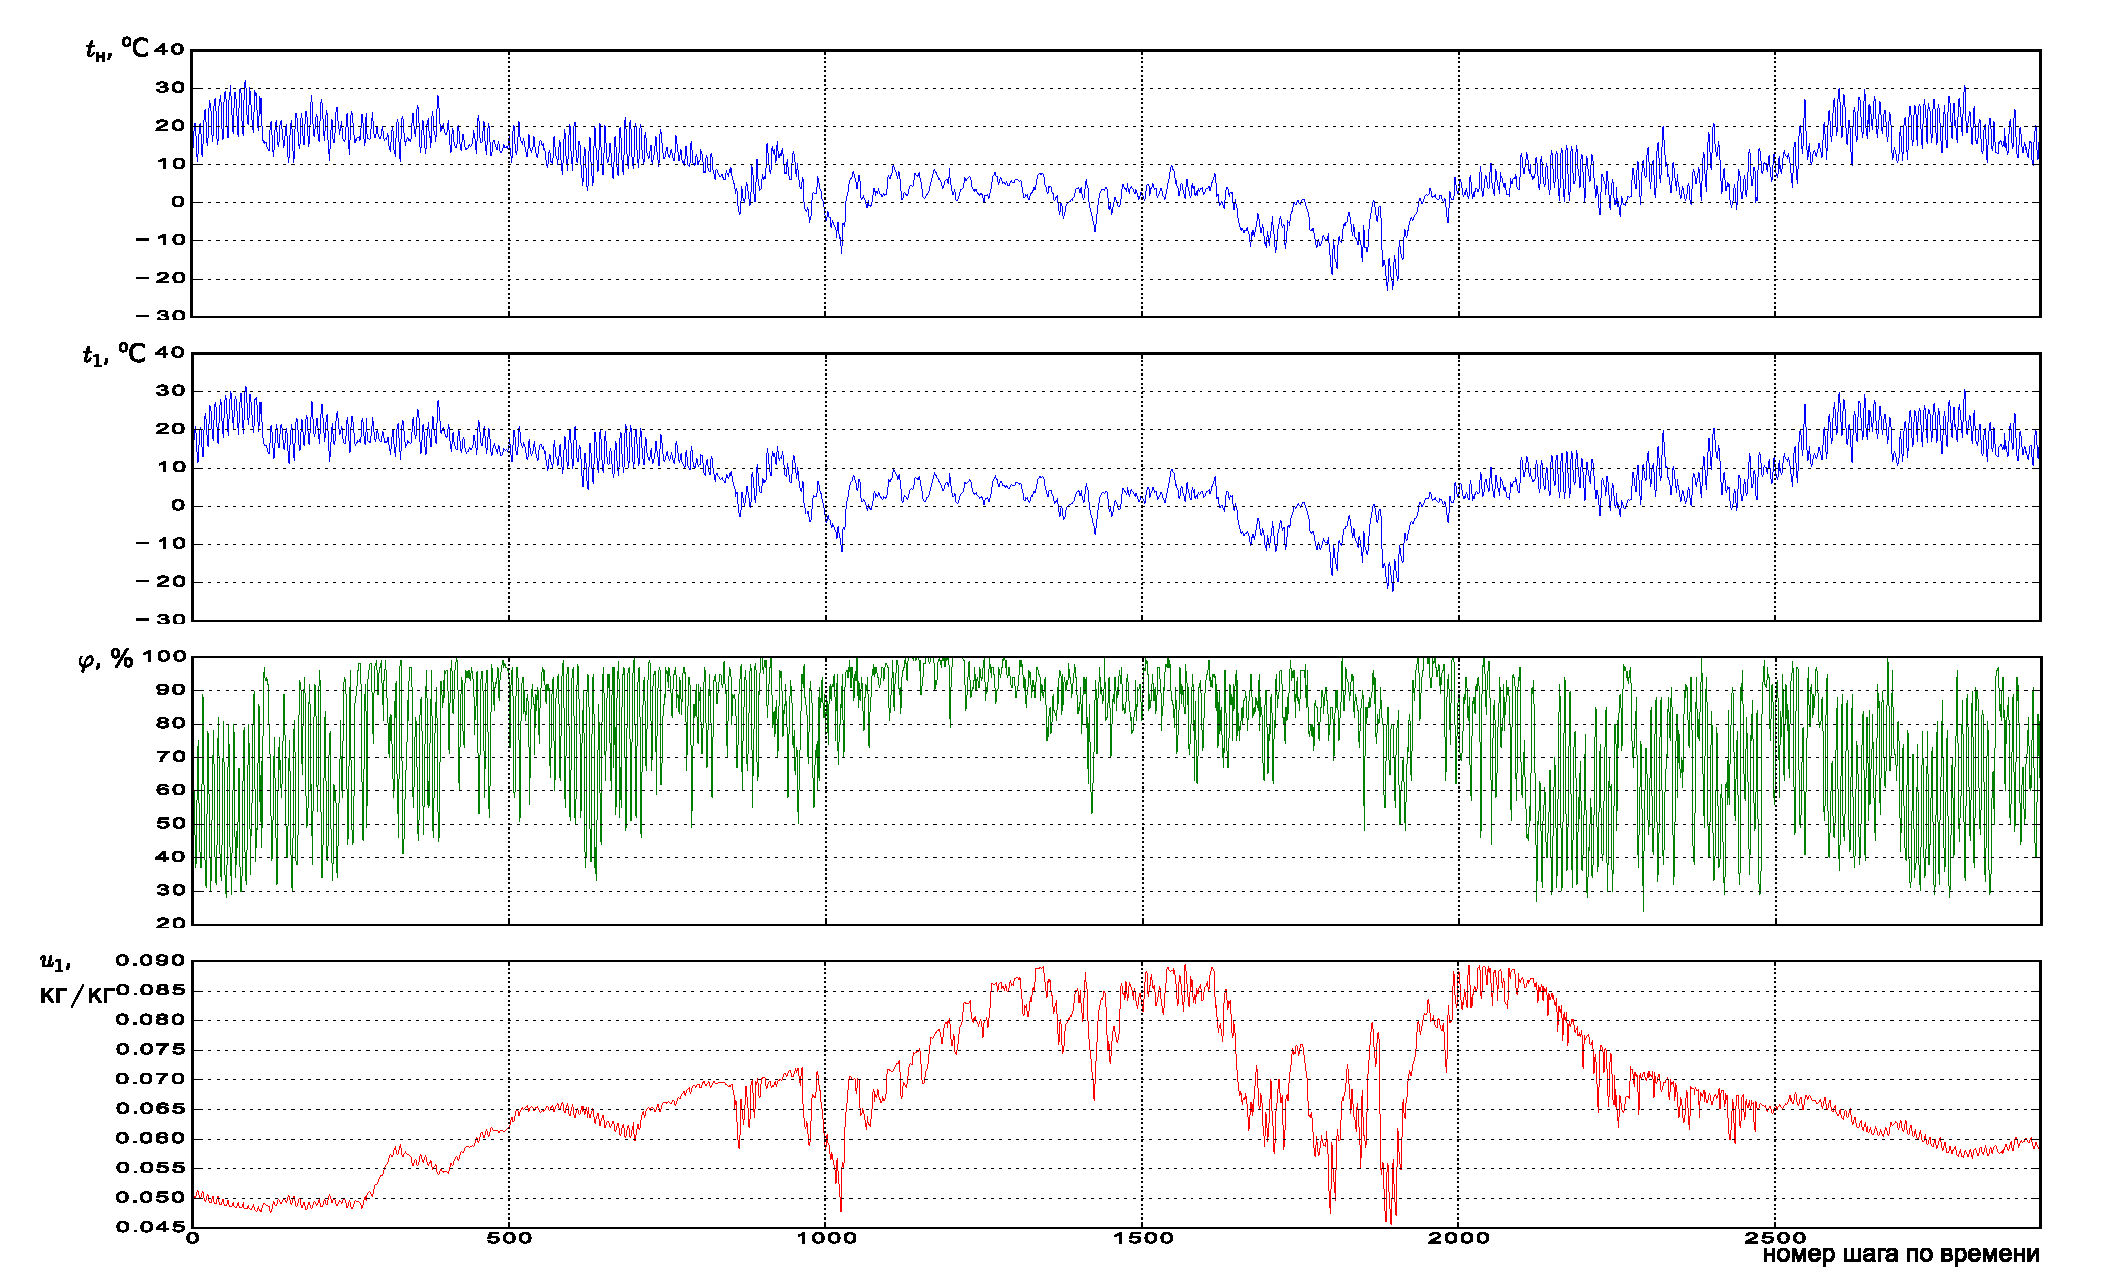
\includegraphics[angle=0,width=1.0\linewidth]{ch5-point1-1}\\[2mm]
\vspace{-10pt}
\caption {Рисунок сделан с помощью Matplotlib}\label{img:point1-1}
\end{center}
\end{figure}

...
